\chapter{Navigation}
Für die Navigation innerhalb der App wurde auf intuitives und simples Design gesetzt, es sollte von
jedem sofort verstanden werden. Natürlich ist das Selbst-Implementieren dieser Funktionalität keine
Option, daher wurde die Bibliothek React Navigation verwendet. Sie verknüpft die einzelnen Screens
der App miteinander und stellt das Gegenstück zu React Router für React im Webbrowser dar.

Damit die Navigation funktionieren kann, muss die gesamte App ein Kind von NavigationContainer sein,
einer Komponente, die von React Navigation importiert wird.

\begin{code}[htp]
\begin{lstlisting}[firstnumber=1,language=JavaScript, style=JSX]
import { NavigationContainer } from '@react-navigation/native';

const App = () => (
  <AuthProvider>
    <NavigationContainer>
      <AuthHandler />
    </NavigationContainer>
    <FlashMessage position="top" />
  </AuthProvider>
);
\end{lstlisting}
\caption{JavaScript Funktion - In NavigationContainer können Navigationen erstellt werden.}
\end{code}

Die Navigation innerhalb der App wurde auf zwei Arten umgesetzt:

\begin{figure}[H]
  \begin{center}
    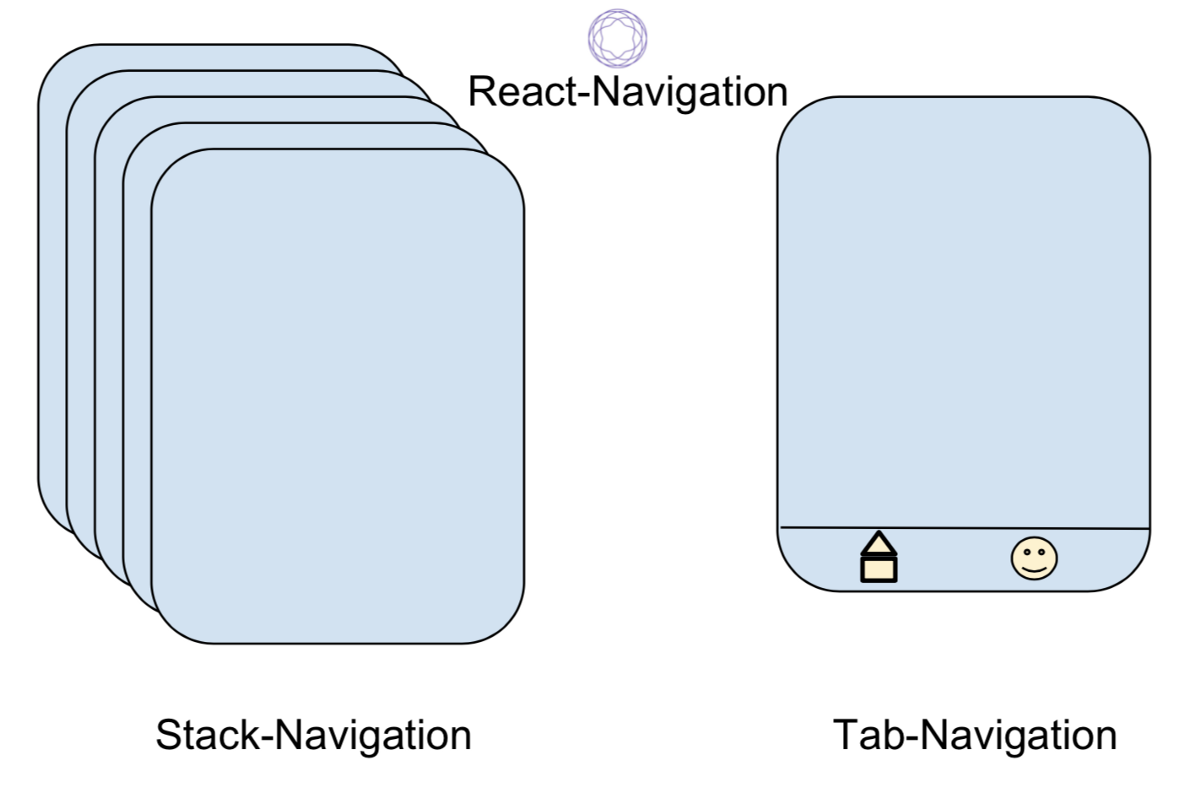
\includegraphics[width=0.5\textwidth]{Mobile/Navigators.png}
    \caption{Stack Navigator und Tab-Navigator}
  \end{center}
\end{figure}

\newpage
\part{Theoretische Grundlagen}

\part{Theoretische Grundlagen}

\part{Theoretische Grundlagen}

\input{parts/2-theorie/1-programmiersprachen/index.tex}
\input{parts/2-theorie/2-haupttechnologien/index.tex}
\part{Theoretische Grundlagen}

\input{parts/2-theorie/1-programmiersprachen/index.tex}
\input{parts/2-theorie/2-haupttechnologien/index.tex}
\part{Theoretische Grundlagen}

\part{Theoretische Grundlagen}

\input{parts/2-theorie/1-programmiersprachen/index.tex}
\input{parts/2-theorie/2-haupttechnologien/index.tex}
\part{Theoretische Grundlagen}

\input{parts/2-theorie/1-programmiersprachen/index.tex}
\input{parts/2-theorie/2-haupttechnologien/index.tex}

\newpage

\part{Theoretische Grundlagen}

\part{Theoretische Grundlagen}

\part{Theoretische Grundlagen}

\input{parts/2-theorie/1-programmiersprachen/index.tex}
\input{parts/2-theorie/2-haupttechnologien/index.tex}
\part{Theoretische Grundlagen}

\input{parts/2-theorie/1-programmiersprachen/index.tex}
\input{parts/2-theorie/2-haupttechnologien/index.tex}
\part{Theoretische Grundlagen}

\part{Theoretische Grundlagen}

\input{parts/2-theorie/1-programmiersprachen/index.tex}
\input{parts/2-theorie/2-haupttechnologien/index.tex}
\part{Theoretische Grundlagen}

\input{parts/2-theorie/1-programmiersprachen/index.tex}
\input{parts/2-theorie/2-haupttechnologien/index.tex}